\documentclass[12pt]{../manual}
%____________________________________________________________________________
%
%	TITLE AND TABLE OF CONTENTS
%____________________________________________________________________________
\begin{document}
\makeheader{Lab 1}
\begin{center}
\textbf{\huge ECE 230L - LAB 1}\\~\\
\textbf{\large LABORATORY ORIENTATION, OPERATION OF DIGITAL INSTRUMENTS, AND BASIC MEASUREMENTS }\\~\\
\rule{6.5in}{0.5mm}\\
\end{center}

\tableofcontents

\listoffigures

\newpage
%____________________________________________________________________________
%
%	BODY
%____________________________________________________________________________
\section{Objectives of this Laboratory}
The objectives of this laboratory session are as follows:
\begin{itemize}
\item To familiarize yourself with the laboratory kit, 
\item To learn to operate the digital instruments, and 
\item To carry out some basic static and dynamic measurements. 
\end{itemize}

\section{ECE 230L Laboratory Introduction}
In this section of the lab, you will familiarize yourself with the laboratory test and measurement equipment available in the ECE 230L Microelectronic Devices and Circuits laboratory.  Take a few minutes to look over the materials included in your laboratory kit and read the descriptions that follow to get acquainted with the devices you will be using all semester in lab. The laboratory kit includes the following instruments:
\begin{itemize}
\item UCTRONICS U6225 Power Supply Module, 
\item Analog Devices M1K ADALM1000,
\item Jameco Breadboard
\item AstroAI AM33D Multimeter
\end{itemize}

\subsection{UCTRONICS U6225 Power Supply Module}
Examine the controls and terminals. This instrument is relatively simple to use. It is used to provide DC (constant) voltages and currents. \textbf{It is important to prevent the leads of the DC power supply from touching each other. When the power supply leads touch, a short circuit is formed which can cause serious damage to the power supply.} Consider what would happen if you shorted the wall socket, or a car battery! Short circuits can be dangerous, and special care should be taken to avoid them.

\begin{figure}[ht!]
\centering
\begin{tabular}{cc}
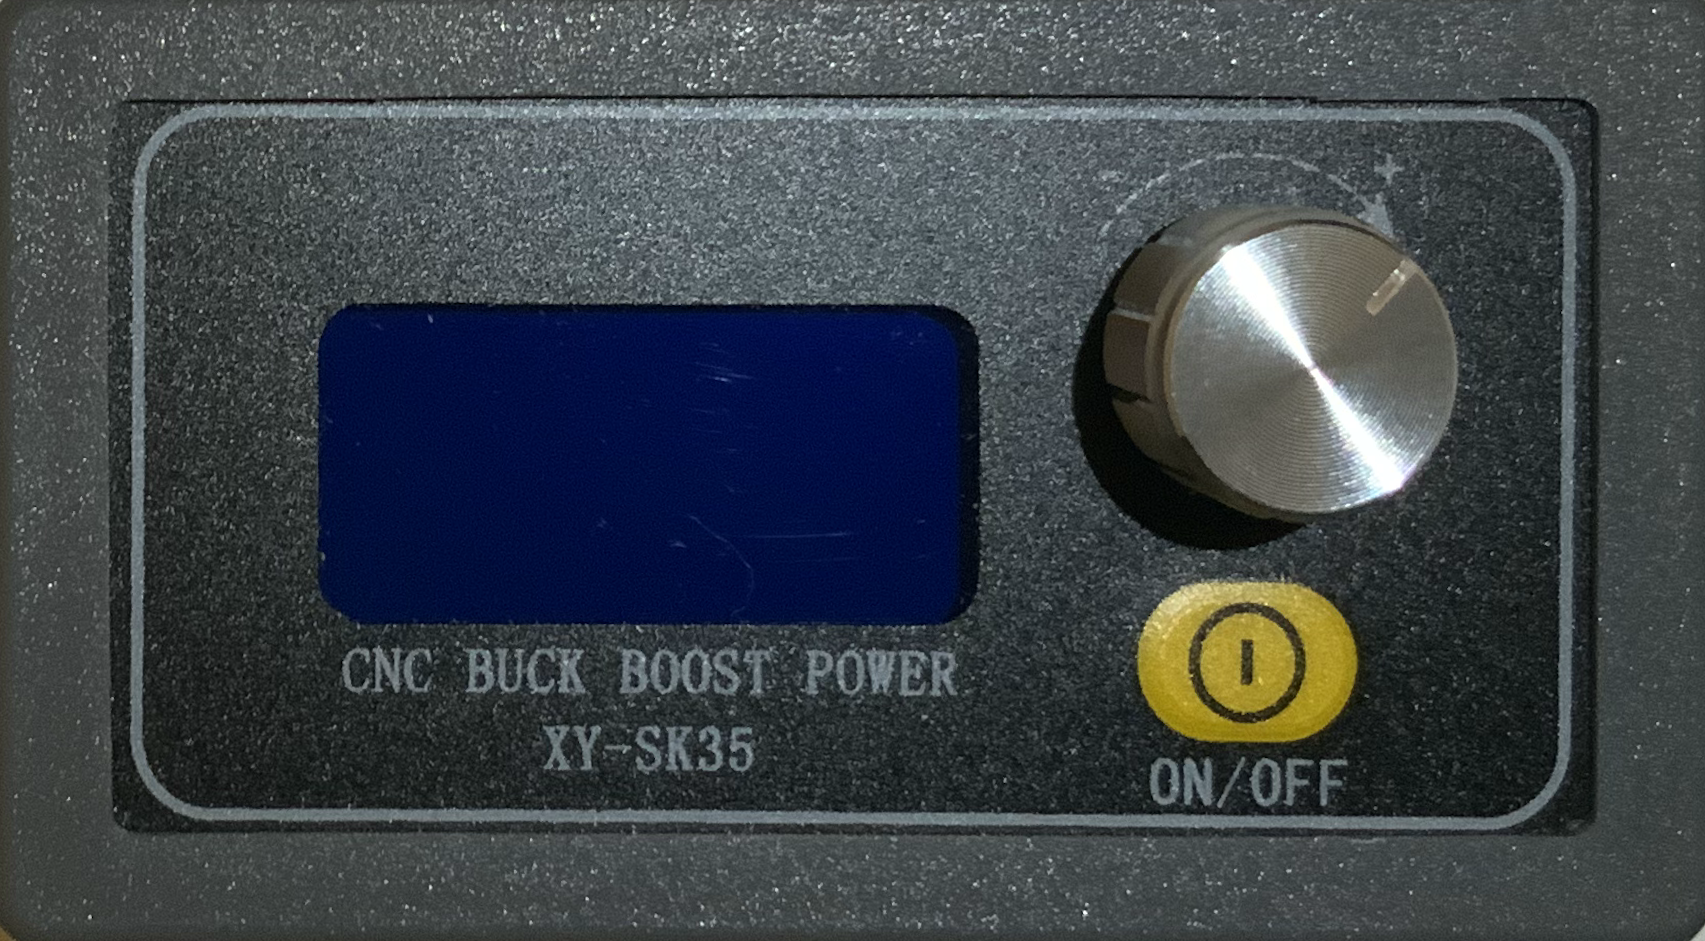
\includegraphics[width=0.4\textwidth]{figures/powerConverterModuleOff.png} & 
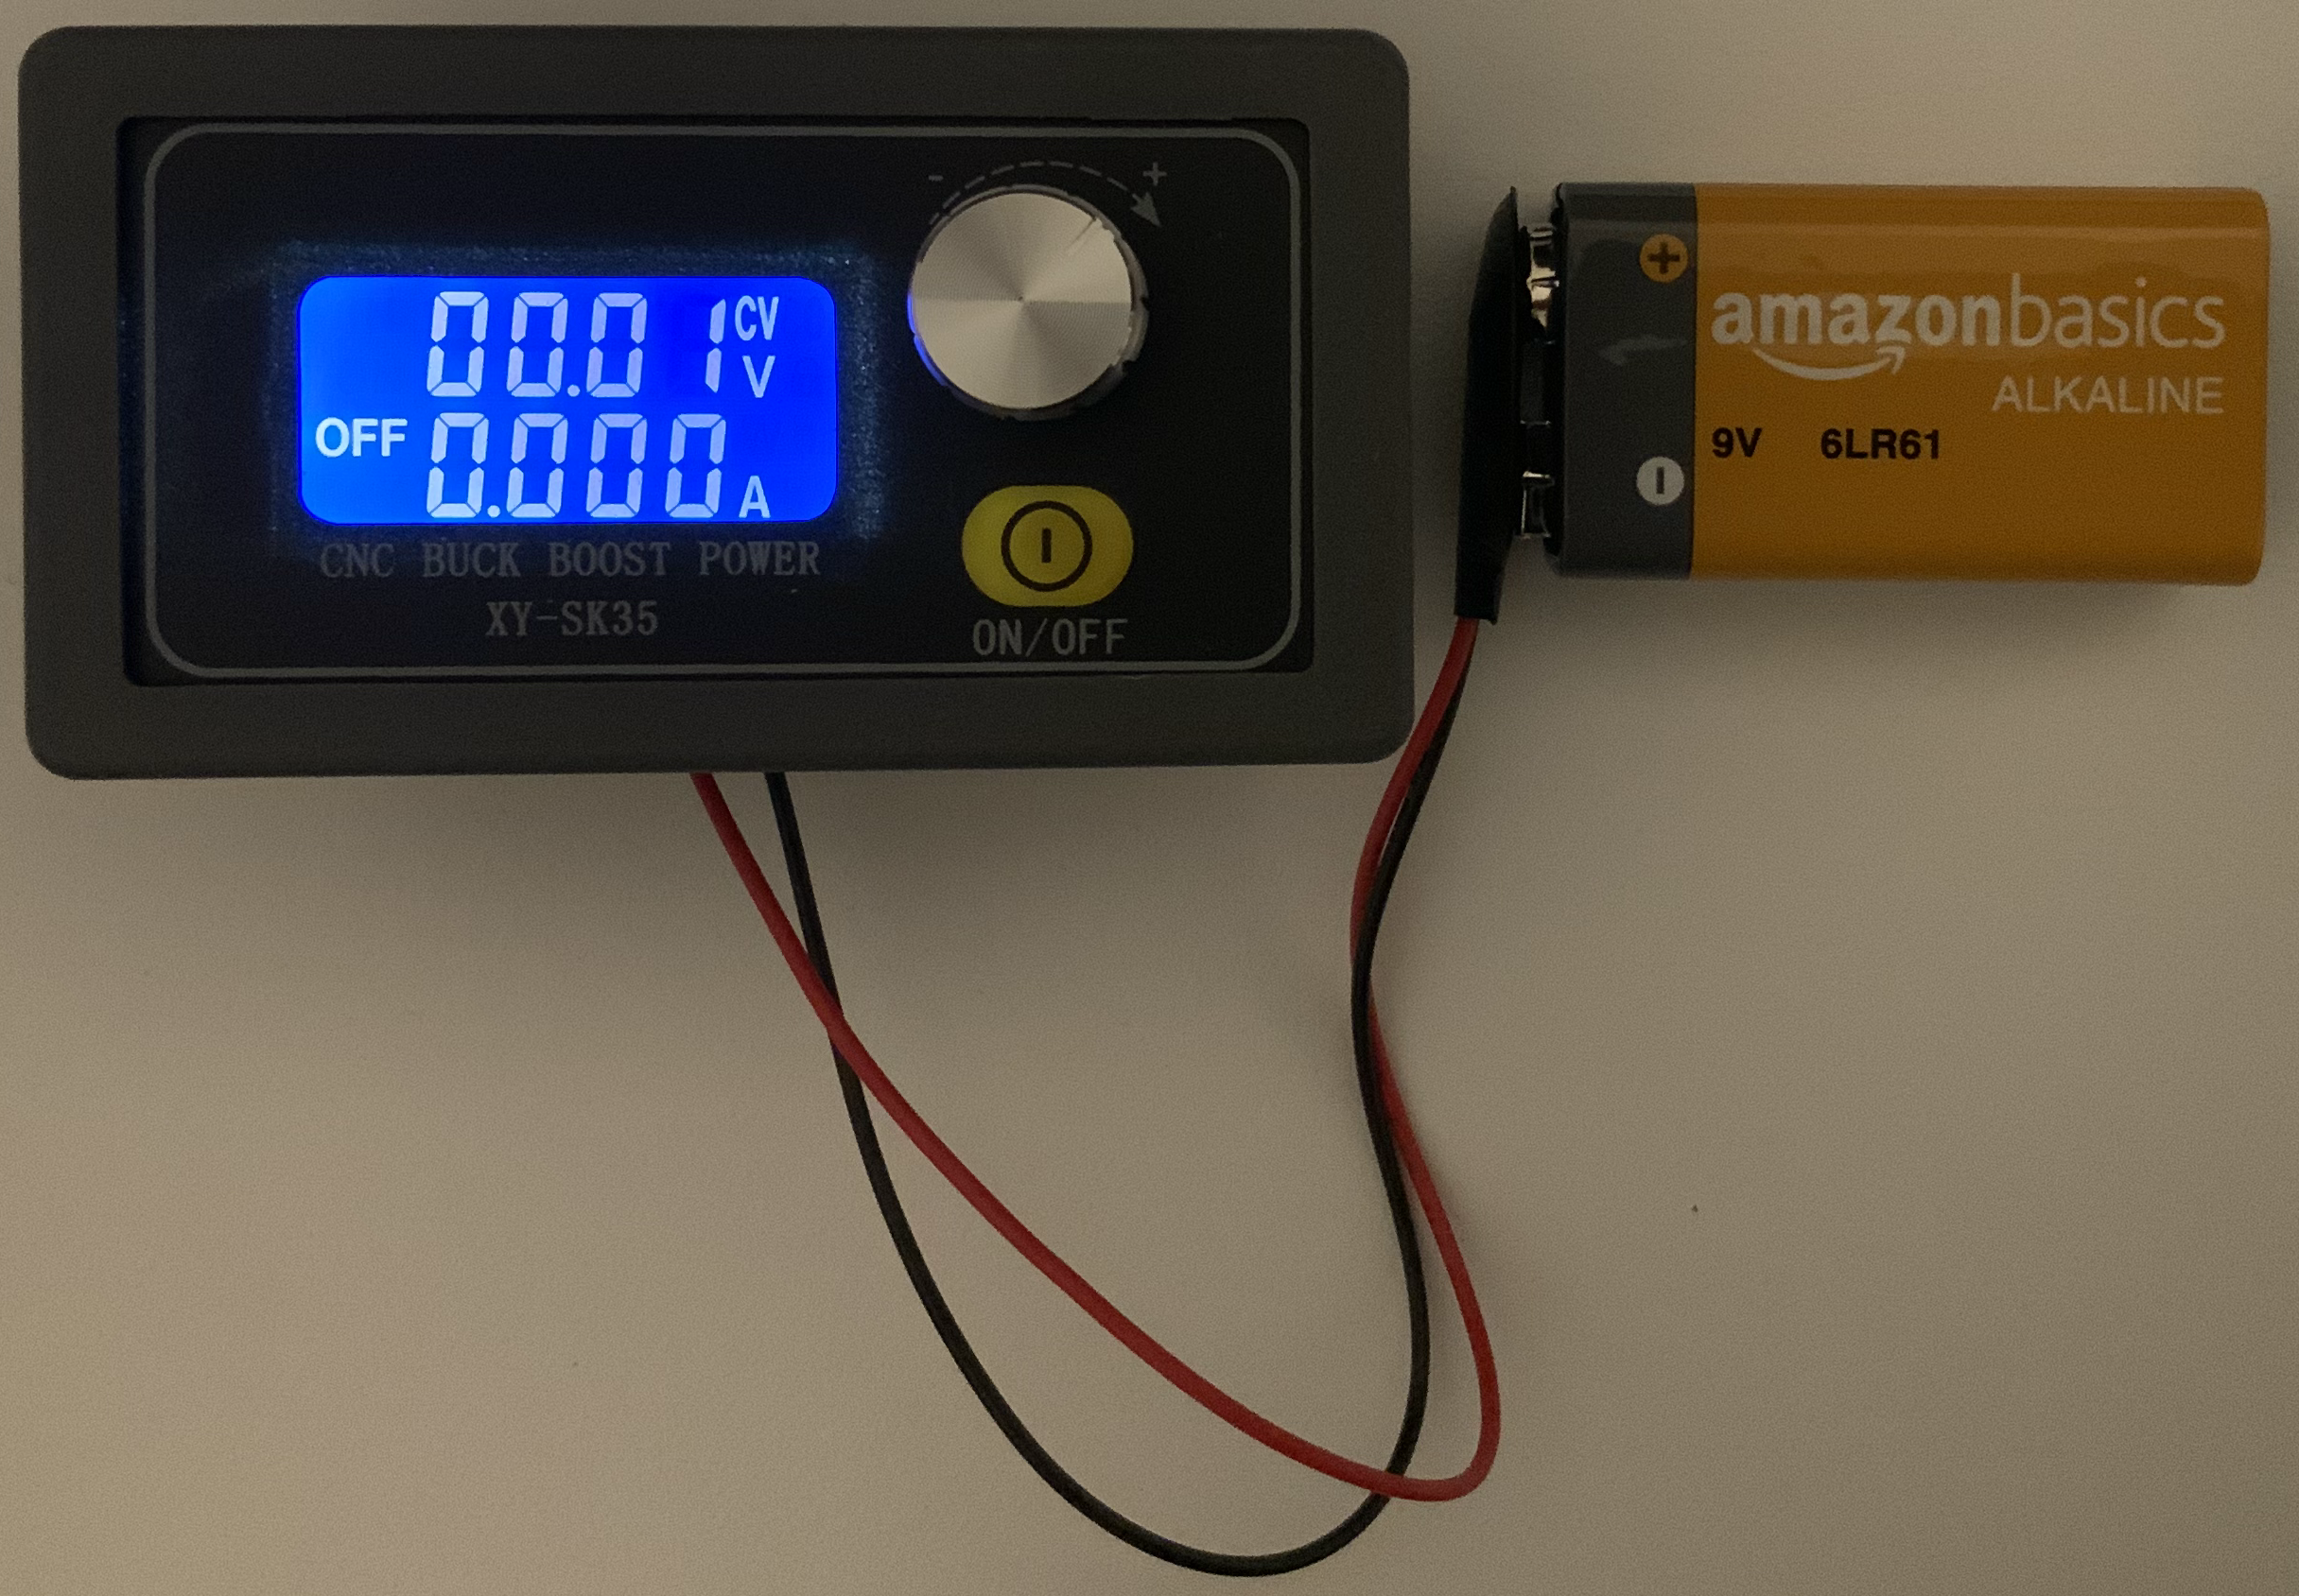
\includegraphics[width=0.4\textwidth]{figures/powerConverterModule.png}
\end{tabular}
\caption[UCTRONICS U6225 Power Supply Module]{Left: Power Supply Module off; Right: Power Supply Module with the positive terminal of the battery plugged in to $V_{IN+}$ and the negative terminal plugged in to $V_{IN-}$}
\label{fig:powerSupply}
\end{figure}

\subsection{Analog Devices M1K ADALM1000}
This instrument is shown in Figure \ref{fig:osc}. This instrument is the most versatile of all the instruments shown because it can perform multiple functions simultaneously. Not only can it act as an oscilloscope, it will also be our function generator for this semester. You can find documentation about the M1K \href{https://wiki.analog.com/university/tools/m1k}{here}.

\begin{figure}[ht!]
\begin{center}
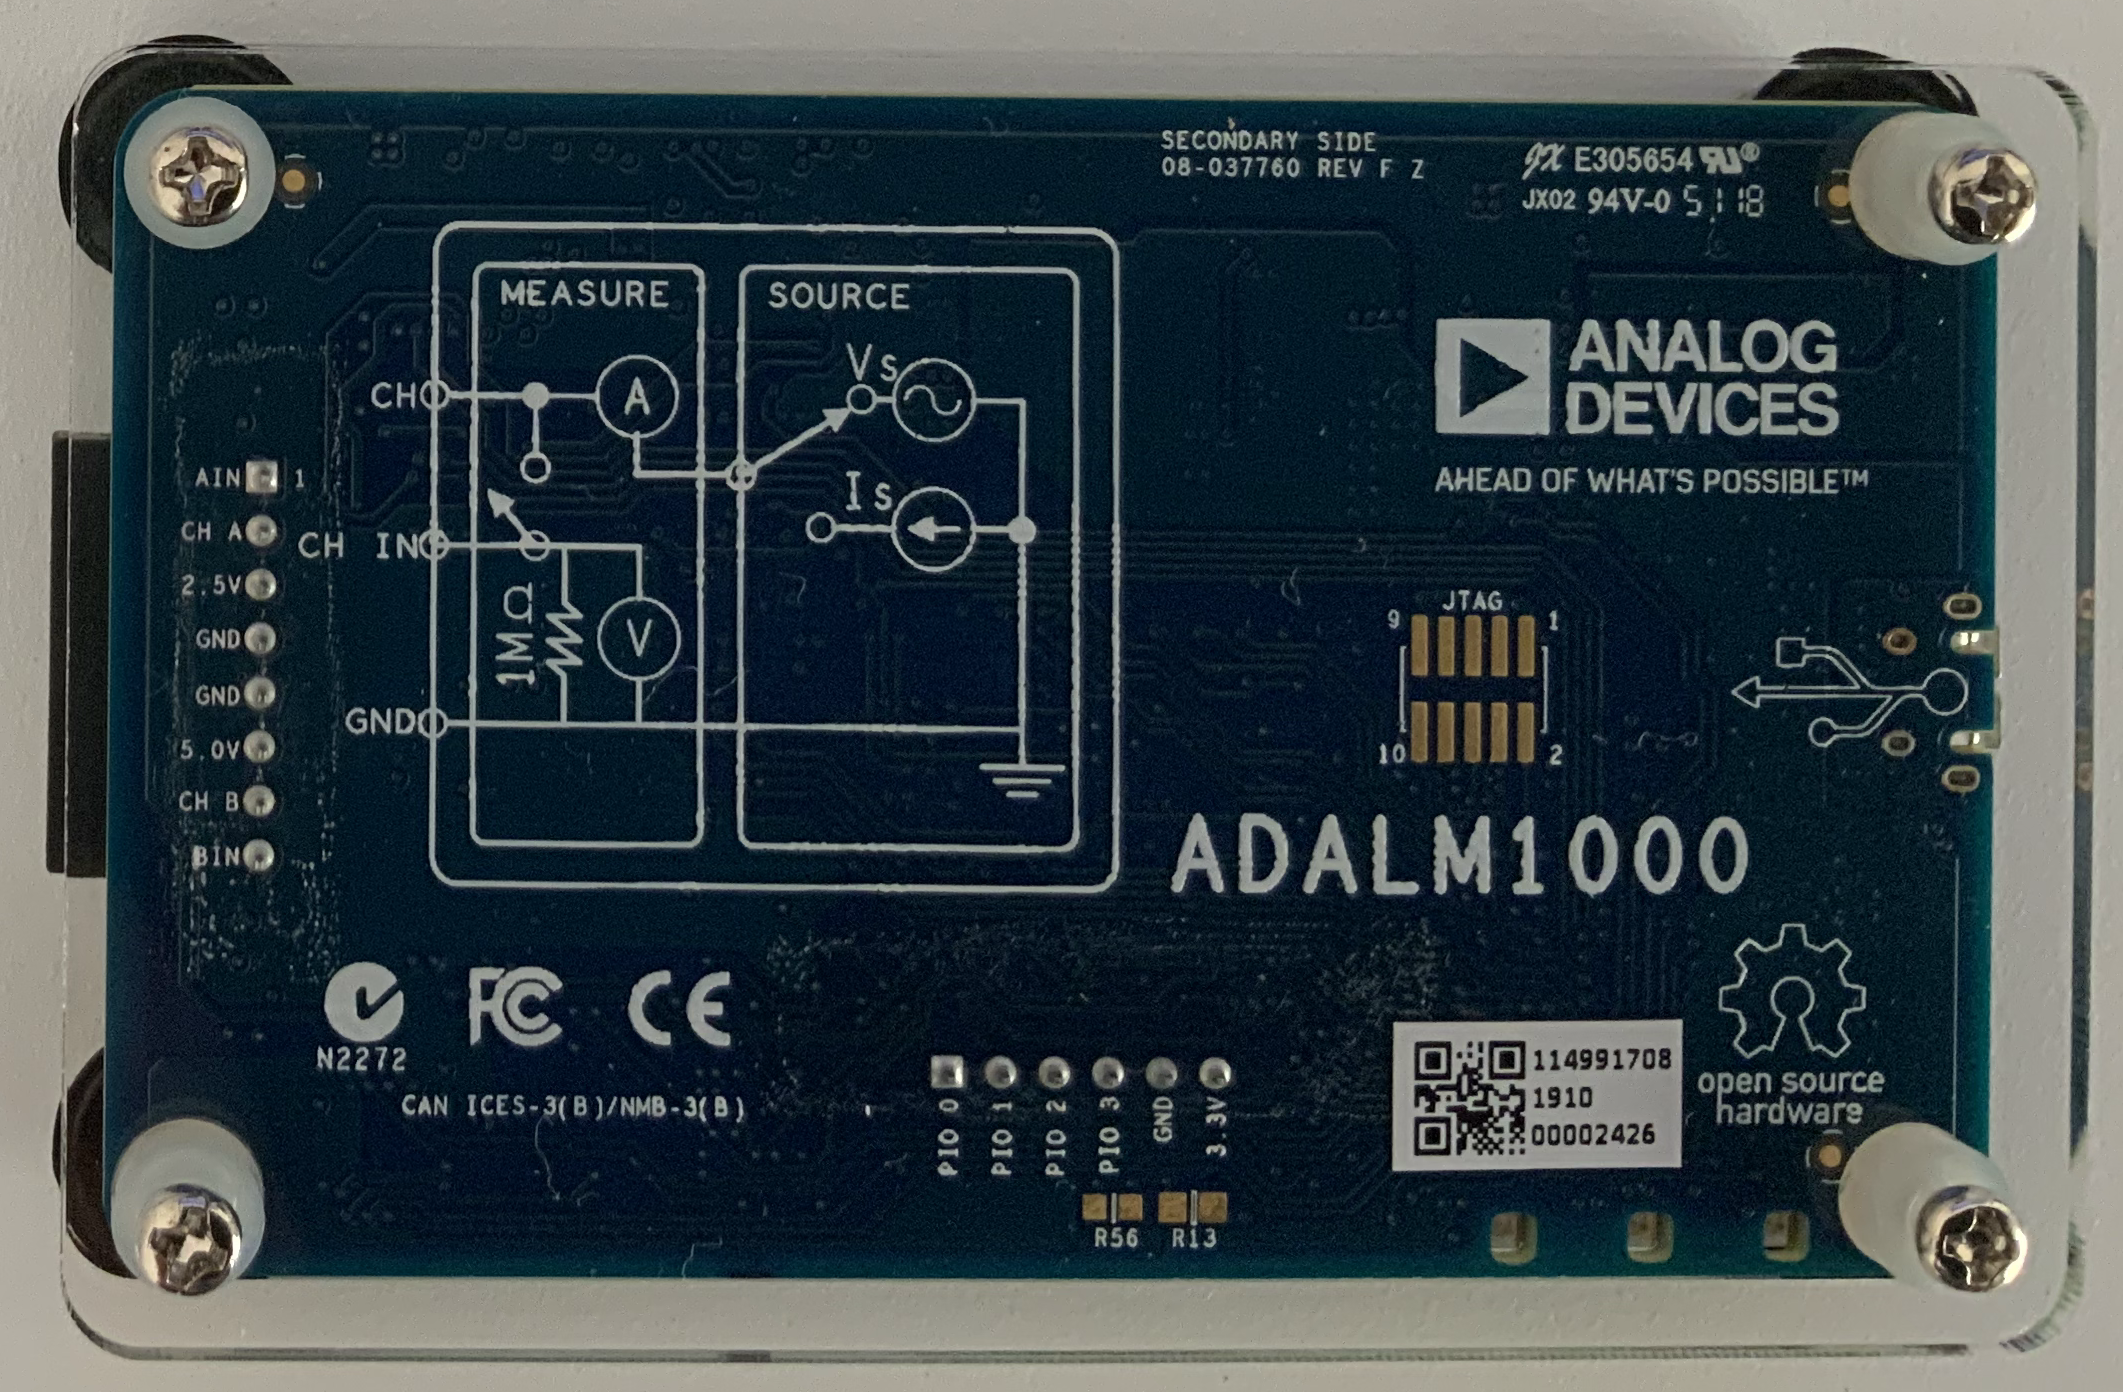
\includegraphics[width=0.5\textwidth]{figures/ADALM1000.png}
\caption[Analog Devices M1K ADALM1000]{Analog Devices M1K ADALM1000}
\label{fig:osc}
\end{center}
\end{figure}

You will be interacting with this instrument through a software called Pixelpulse2. Instructions on how to download Pixelpulse2 are included in Section 3.

\subsection{Jameco Breadboard}
You've probably seen this exact breadboard model in your previous ECE laboratories. You will be using this breadboard to build most of your circuits. Remember that any components placed in a row will be electrically connected to anything else placed in that row.

\begin{figure}[ht!]
\begin{center}
\includegraphics[width=0.4\textwidth, angle=90]{figures/breadboard.png}
\caption[Jameco Breadboard]{Jameco Breadboard}
\label{fig:breadboard}
\end{center}
\end{figure}

\subsection{AstroAI AM33D Multimeter}
This instrument is used to measure voltages, currents, and resistances. When configured to measure voltage, it is a voltmeter. When configured to measure current, it is an ammeter. When configured to measure resistance, it is an ohmmeter. Remember, you may have to change the terminal that the red lead is connected to in order to make certain measurements. 

\begin{figure}[ht!]
\begin{center}
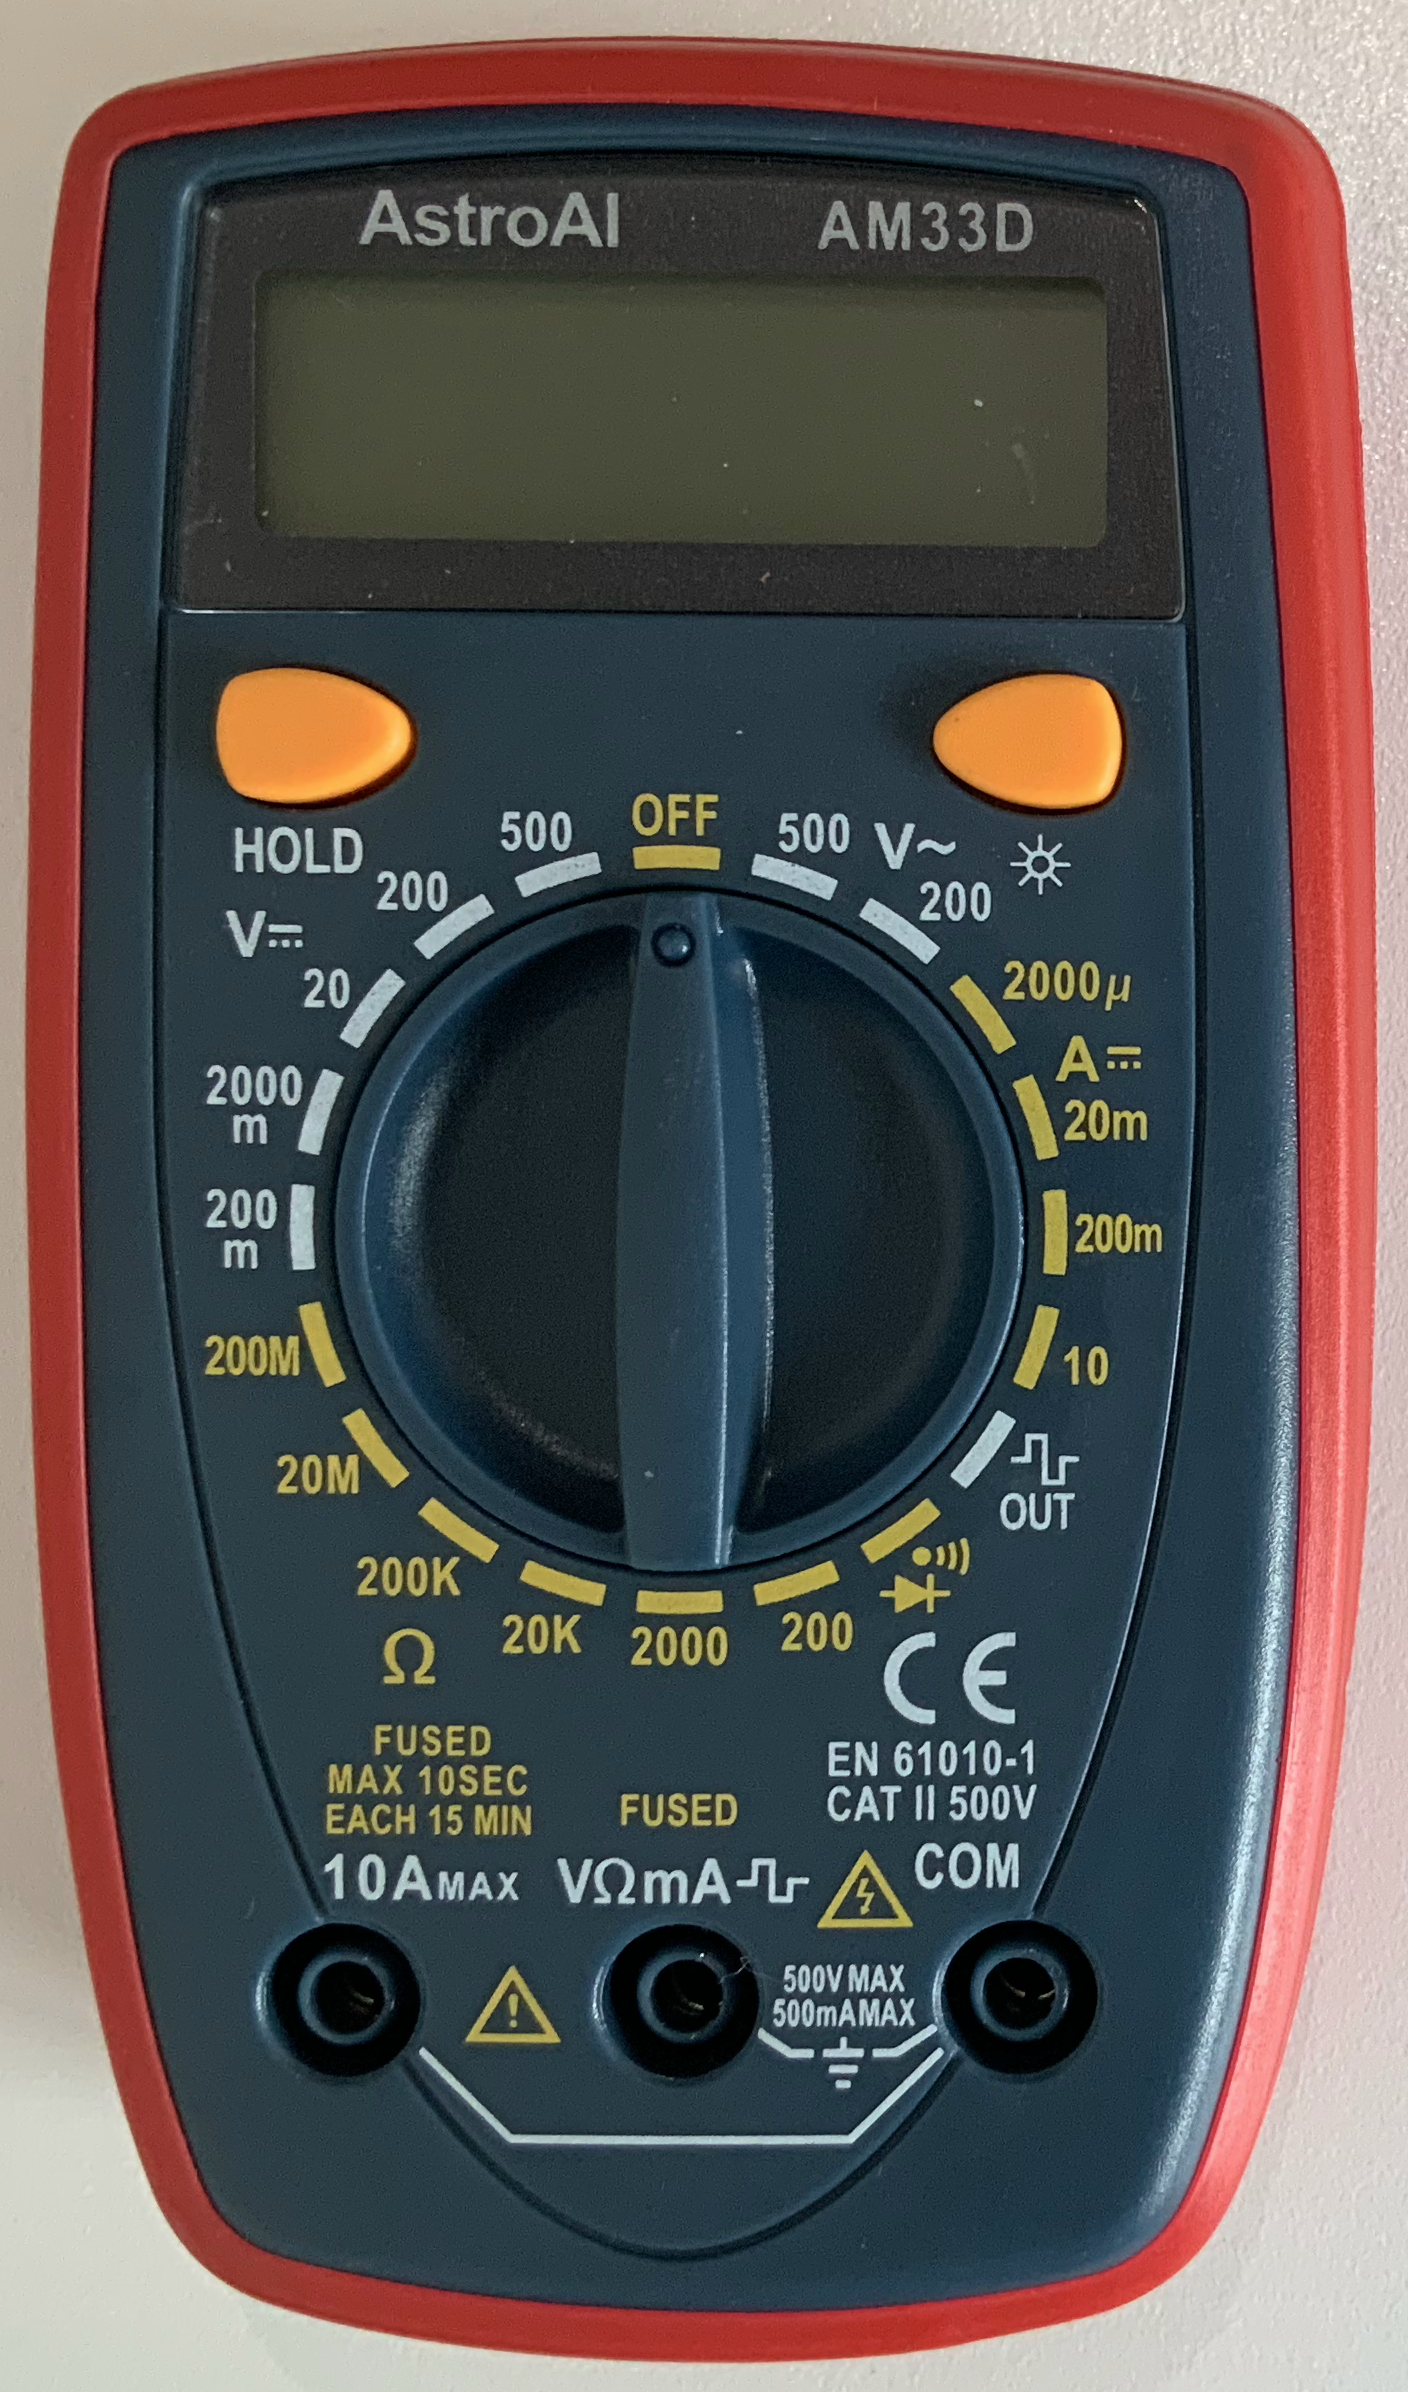
\includegraphics[width=0.4\textwidth]{figures/multimeter.png}
\caption[AstroAI AM33D Multimeter]{AstroAI AM33D Multimeter}
\label{fig:multimeter}
\end{center}
\end{figure}

\newpage
\section{Laboratory Preparation}
\subsection{Download and Install Pixelpulse2}
You can find the download link for Pixelpulse2 \href{https://github.com/analogdevicesinc/Pixelpulse2/releases/tag/v1.0.4}{here}. If you are on a Windows device, download {\tt Pixelpulse2\_win\_setup.exe}. If you are on a Mac, download {\tt Pixelpulse2-v1.0.4.dmg.zip}. After following the installation instructions, open Pixelpulse2. Confirm your application looks like the image below.

\begin{figure}[ht!]
\begin{center}
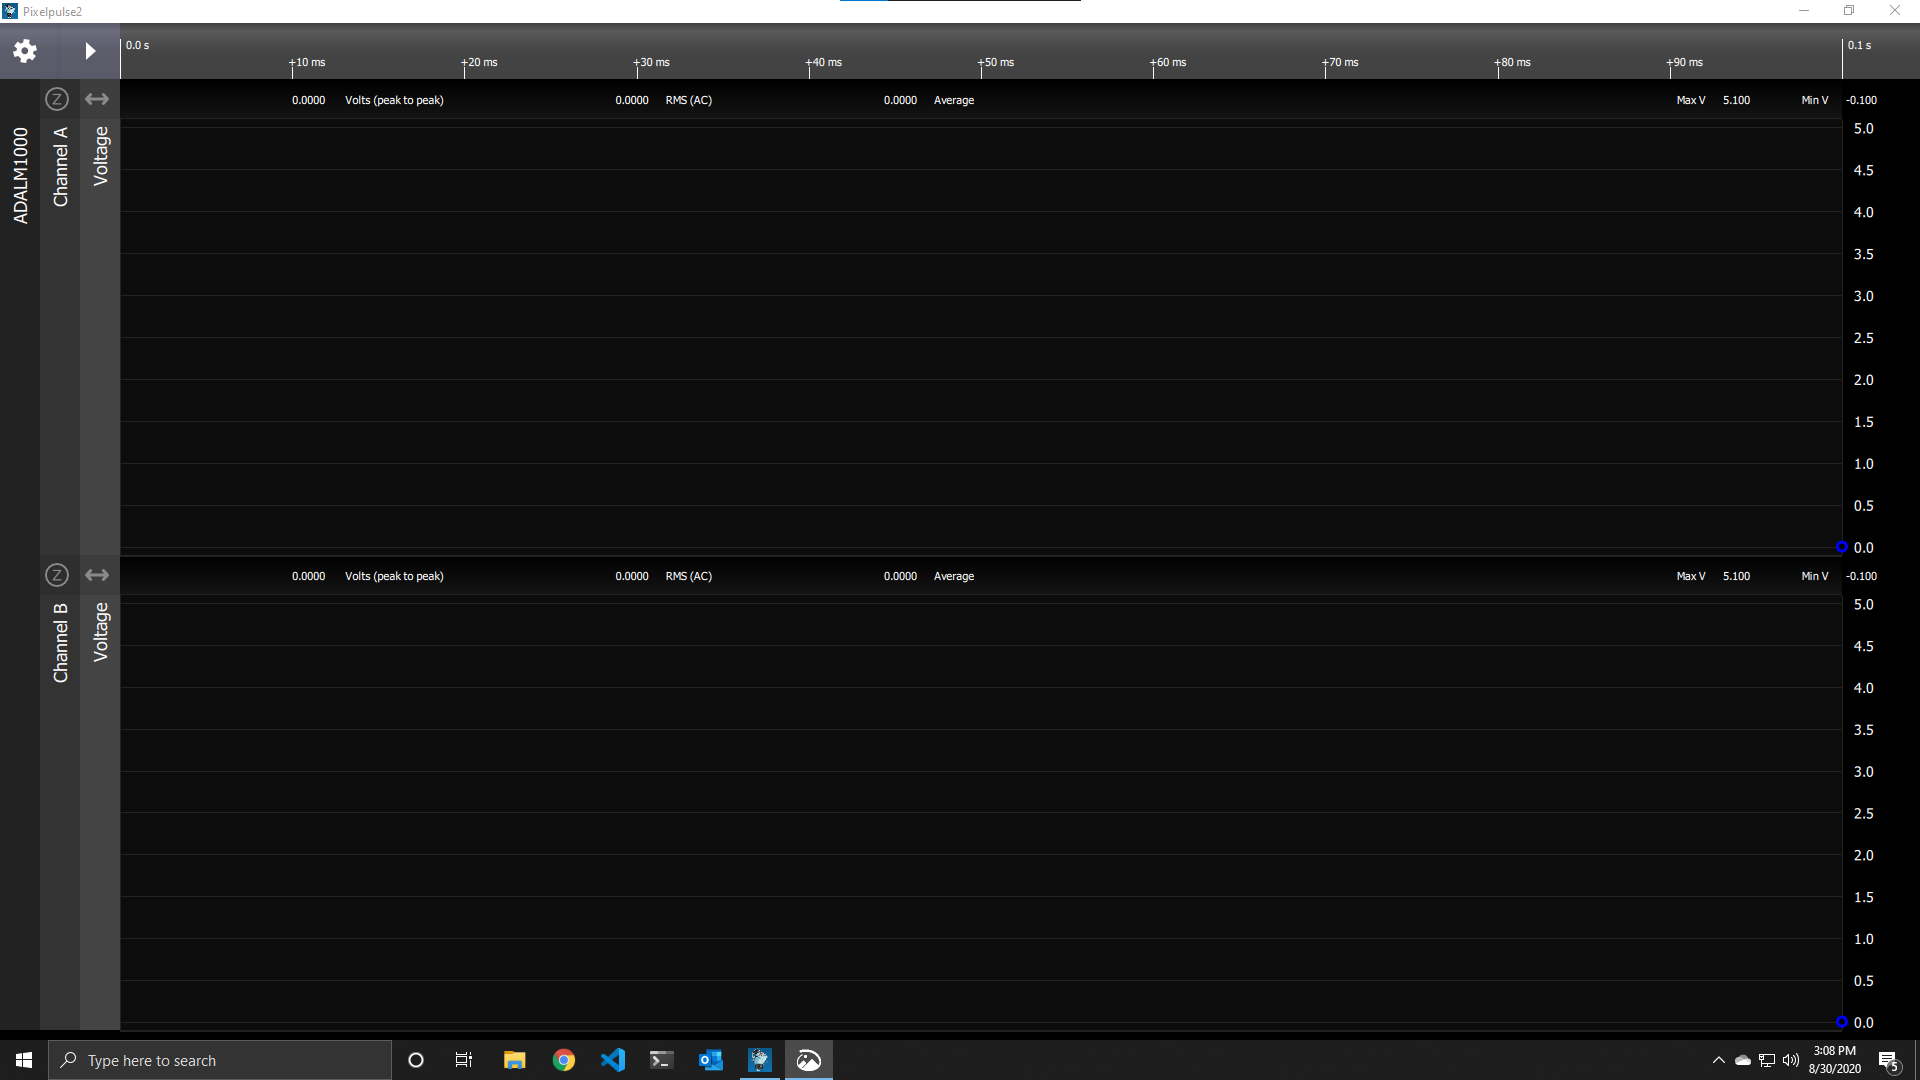
\includegraphics[width=0.9\textwidth]{figures/Pixelpulse2.png}
\caption[Pixelpulse2 GUI]{Pixelpulse2 GUI}
\label{fig:pixelpulse2}
\end{center}
\end{figure}

Note that you may have to update your device's firmware the first time you open the application. This should only take a few seconds. Unplug and plug the M1K back in once you receive a message saying that the firmware has been updated.

Also, you may want to check out \href{https://wiki.analog.com/university/tools/m1k/pixelpulse}{the wiki}.

\newpage
\section{Experimental Exercises}
\subsection{Practical Voltage and Current Measurements}
The standard resistor color code is shown on the wall in the laboratory above your lab bench. Most resistors have four colored bands. The first three bands indicate the nominal value of the resistor and the fourth band indicates the tolerance in its value. The first two bands form the mantissa and the third band represents the power of 10. A table of the resistance color code is included below for your convenience.

\def\arraystretch{1.4}
\begin{table}[ht!]
\caption{Resistance Color Code}
\centering
\begin{tabular}{|c|c|c|} \hline
Color 	& Mantissa Value & Multiplier \\ \hline \hline
Black 	& 0 & $10^0$ \\ \hline
Brown 	& 1 & $10^1$ \\ \hline
Red 	& 2 & $10^2$ \\ \hline
Orange 	& 3 & $10^3$ \\ \hline
Yellow	& 4 & $10^4$ \\ \hline
Green	& 5 & $10^5$ \\ \hline
Blue	& 6 & $10^6$ \\ \hline
Violet	& 7 & $10^7$ \\ \hline
Grey	& 8 & $10^8$ \\ \hline
White	& 9 & $10^9$ \\ \hline
\end{tabular}
\end{table}

The tolerance band is typically either Gold or Silver. A Gold tolerance band indicates that the measured value will be within 5\% of the nominal value. A Silver band indicates a 10\% tolerance. For example, a resistor with color code brown-black-red-silver indicates a nominal value of 1 k$\Omega$. The first two bands (Brown followed by Black) produce the mantissa of 10 and the third band (Red) is the exponent of two $(10^2 = 100)$. Therefore, the value of a brown-black-red-silver resistor is $10 \times 100 = 1$ k$\Omega$. Because the tolerance band is Silver, we can expect the measured value of the resistor to be between 900 and 1100 $\Omega$. 

\subsubsection{Ideal vs. Practical DC Voltmeters}
An ideal voltmeter has an infinite series resistance, i.e., it is practically an open circuit. Although it is impossible to make a physical voltmeter with infinite resistance, a well designed voltmeter exhibits a very large internal resistance. In some experiments, it is important to take into account the finite, non-ideal internal resistance of a DC voltmeter.

To determine the internal resistance of the voltmeter, set up a circuit as shown in Figure \ref{fig:voltcirc}.

\begin{figure}[ht!]
\begin{center}
\begin{circuitikz}[american, scale=1.5]
\ctikzset{resistors/scale=1.5, batteries/scale=1.5, instruments/scale=1.5}
\draw 
(0,0) to [resistor, l_=\SI{1}{M\ohm}, *-] ++(-3,0)
to [battery, l_=\SI{10}{V}] ++(0,-2)
to [short, -*] ++(3,0)
(0.25,-2) node[currarrow, rotate=180]{}
to [short] ++(0.75,0)
to [rmeter, t=V] ++(0,2)
to [short] ++(-0.75,0) node[currarrow, rotate=180]{}
;\end{circuitikz}
\caption[Circuit used to measure internal resistance of voltmeter]{Circuit used to measure the internal resistance $R_M$ of the voltmeter}
\label{fig:voltcirc}
\end{center}
\end{figure}

Note that you may need to use the 2.4 mm screwdriver to loosen and tighten the terminals of the power supply.

The voltmeter reads the voltage across itself, which includes its internal resistance. Because the circuit has only a single branch, the current flowing through the resistor also flows through the voltmeter. In this circuit, the source voltage $V_S = 10$ V and the DC voltage measured by the voltmeter is $V_M$. The current is given by the equation
\begin{align}
I = \frac{V_S - V_M}{R}.
\end{align}
From Ohm's Law, if we measure the current I and the voltage $V_M$, we can determine the resistance, $R_M$ of the voltmeter from 
\begin{align}
R_M = \frac{V_M}{I} = \frac{V_M}{\frac{V_S - V_M}{R}} = \frac{V_M}{V_S - V_M}R
\end{align}
To determine the internal resistance of the voltmeter, carry out the following steps:
\begin{enumerate}
\item Select a 1 M$\Omega$ resistor. 
\item Measure its resistance using the multimeter. 
\item Set the power supply to provide 10 V. Always remember to measure the voltage provided by the power supply either with the voltmeter or the scope. Do not rely on the digital display on the front panel of the power supply. 
\item Assemble the circuit in Figure \ref{fig:voltcirc}. 
\item Record the voltage $V_M$ measured by the voltmeter. 
\item Compute the internal resistance $R_M$ of the voltmeter (above) 
\end{enumerate}

\subsubsection{Ideal vs. Practical DC Ammeters}
An ideal ammeter has zero internal resistance so that the circuit in which it has been placed is not disturbed. An ideal ammeter is a short circuit. As with the voltmeter, however, no ammeter is ideal. Thus, all ammeters have some optimally small internal resistance.

To determine the resistance of the DC ammeter, set up a circuit as shown in Figure \ref{fig:ampcirc}.

\begin{figure}[ht!]
\begin{center}
\begin{circuitikz}[scale=1.5]
\ctikzset{resistors/scale=1.5, batteries/scale=1.5, instruments/scale=1.5}
\draw 
(0,0) to [resistor, l_=\SI{100}{\ohm}] ++(-4,0)
to [battery, l_=\SI{1}{V}] ++(0,-2)
to ++(4,0) 
to [rmeter, t=A] ++(0,2)
;\end{circuitikz}
\caption[Circuit used to measure internal resistance of ammeter]{Circuit used to measure the internal resistance $R_M$ of the ammeter}
\label{fig:ampcirc}
\end{center}
\end{figure}

According to Ohm's Law, the current in this circuit is given by
\begin{align}
I = \frac{V_S}{R + R_M}
\end{align}
By measuring the current $I$ and the source voltage $V_S$, and knowing the value of the series resistance $R$, we can determine the ammeter resistance $R_M$ from
\begin{align}
R_M = \frac{V_S}{I} - R \label{eq:amres}
\end{align}
In the procedure that follows, it is extremely important that you take precise and accurate measurements. Record each measurement as precisely as the instrument will allow.
\begin{enumerate}
\item Select a 100 $\Omega$ resistor. Measure and record its resistance. 
\item Set the voltage of the DC Voltage Source to 1 V.
\item Assemble the circuit shown in Figure \ref{fig:ampcirc}. Set the multimeter to the ammeter mode for DC current measurement.
\item Use the oscilloscope to measure the voltage $V_S$ across the DC power supply (use the ``average'' measurement).
\item Measure the DC current $I$ using the ammeter. 
\item Determine the value of $R_M$ from Equation \eqref{eq:amres}. 
\end{enumerate}

\newpage
\subsection{Measurements of Time-Dependent Sources}
In this section, we will be using the M1K as a function generator to provide a time-dependent voltage waveform which will then be measured using the other channel of the M1K. \textbf{It is important NOT to let the leads of the M1K touch each other.} If the function generator leads touch each other, either the internal fuse will blow or serious damage to the instrument will occur. If the internal fuse blows, the device will need to be replaced.

During these next few experiments, you will be using Pixelpulse2 to generate three different waveforms: a sine wave, a triangle wave, and a square wave. 

{\bf Setup}
\begin{enumerate}
\item connect the Ch A terminal and GND to the Ch B terminal and GND
\item turn on the function generator by clicking on the ``Z'' above Channel A and selecting ``Source Voltage; Measure Current'' from the drop down menu.
\end{enumerate}

\subsubsection{Sinusoidal Waveform}
\begin{enumerate}
\item Set the function generator to produce a sine wave by clicking on the button above ``Voltage'' and choosing ``Sine''
\item Set the sine wave parameters to the following: 
\begin{itemize}
\item 10 Hz
\item 5 V amplitude
\end{itemize}
\item Change ``Sample Time'' to ``1 s''
\item \textbf{Capture the Pixelpulse2 screen for the entire 1 second interval} and save it to document your laboratory experiments.
\end{enumerate}

\subsubsection{Square Waveform}
\begin{enumerate}
\item Set the function generator to produce a square wave by clicking on the button above ``Voltage'' and choosing ``Square''
\item Set the square wave parameters to the following: 
\begin{itemize}
\item 1 kHz
\item 1.5 V Min
\item 3.0 V Max
\item 75\% duty cycle
\end{itemize}
\item Change ``Sample Time'' to ``10 ms''
\item \textbf{Capture the Pixelpulse2 screen for a 5 ms interval} and save it to document your laboratory experiments.
\end{enumerate}

\subsubsection{Triangle Waveform}
\begin{enumerate}
\item Set the function generator to produce a square wave by clicking on the button above ``Voltage'' and choosing ``Triangle''
\item Set the triangle wave parameters to the following: 
\begin{itemize}
\item 25 Hz
\item 1.0 V Min
\item 4.0 V Max
\end{itemize}
\item Change ``Sample Time'' to ``100 ms''
\item \textbf{Capture the Pixelpulse2 screen for entire 100 ms interval} and save it to document your laboratory experiments.
\end{enumerate}

\newpage
\section{Questions}
\begin{enumerate}
\item Define and differentiate between precision, accuracy, and resolution in electrical measurements. What is the ``resolution'' of your handheld multimeter's display? Why is it a good idea to use the multimeter in conjunction with the DC supply?
\item Look up the internal resistances for both the voltmeter and ammeter capabilities for the AstroAI Digital Multimeter in your lab kit. How do these values compare to the internal resistances you measured in section 3.1? Give percent errors.
\item Suppose you want to produce a 5 V constant voltage across a 500 k$\Omega$ resistor with the M1K. When you do so, what voltage do you expect to measure across your handheld multimeter and why? 
\item Visit the \href{https://wiki.analog.com/university/tools/m1k}{wiki} for the M1K. Access the hardware manual. What is the maximum voltage that can be output by the M1K? Notice that Analog Devices claims that the precision of the M1K can be as small as 10 $\mu$S. What frequency would this be? In Pixelpulse2, what is the maximum frequency you are able to produce? Why do you think that, in practice, the M1K is limited in frequency to only this value?
\end{enumerate}
Submit the answers to these questions along with an extension and all of the other below-listed items in the rubric in your Lab 1 write-up in order to receive all possible points. 

\textit{Laboratory Notebooks:  There is no laboratory notebook requirement in ECE 230L, however, the use of a notebook for recording work performed in the laboratory is a very good practice and one that is encouraged.  Tips and pointers on how to maintain an excellent laboratory notebook are available on the lab site or can be obtained by speaking with your TA or instructor. It is a great idea to add comments and notes to your notebook before leaving lab---this is best done while the work is fresh in your mind!}
\newpage
\section{Extension}
To earn up to an additional 7 points (bringing the total possible points up to 100), you must show evidence of independent thought. This may include (but is not limited to):

In this laboratory, you explored several different devices that you will be using throughout the semester: UCTRONICS U6225 Power Supply Module, Analog Devices M1K ADALM1000, Jameco Breadboard, and AstroAI AM33D Multimeter. Choose one of these devices to explore in greater depth. Consider at least three features of the device you chose to explore. Answers in bullet points are fine. 100 words or less.

You may also choose to explore any other aspect of this laboratory that piqued your interest.

The number of additional points awarded depends on the quality and extent of your independent contribution.

%____________________________________________________________________________
%
%	Grading Rubric
%____________________________________________________________________________
\newpage
\phantomsection
\addcontentsline{toc}{section}{Grading Rubric}
\markboth{Grading Rubric}{Grading Rubric}
\hspace{0pt}
\vfill
\begin{table}[ht!]
\caption{ECE 230L Laboratory 1 Grading Rubric}
\centering
\begin{tabular}{l|c} \hline
Criteria & Points Possible \\ \hline \hline
\textbf{Internal Resistance of a Voltmeter}			& \textbf{10} \\
Circuit Diagram												& 3 \\
Actual measurements for $V_M, V_S$, and $R$			& 3 \\
Equation and $R_M$ value									& 4 \\ \hline
\textbf{Ideal vs. Practical DC Ammeter}				& \textbf{11} \\
Circuit Diagram												& 3 \\
Actual measurements for $V_M, V_S,$ and $R$			& 4 \\
Equation and $R_M$ value									& 4 \\ \hline
\textbf{Measurements of Time-Dependent Sources}		& \textbf{12} \\
Image of sinusoidal waveform								& 4 \\
Image of square waveform									& 4 \\
Image of triangle waveform 								& 4 \\ \hline
\textbf{Question 1}											& \textbf{15} \\ \hline
\textbf{Question 2}											& \textbf{15} \\ \hline
\textbf{Question 3}											& \textbf{15} \\ \hline
\textbf{Question 4}											& \textbf{15} \\ \hline
\textbf{Extension}											& \textbf{7} \\ \hline
\textbf{Total}												& \textbf{100} \\ \hline
\end{tabular}
\end{table}
\vfill
\hspace{0pt}
%____________________________________________________________________________
%
%	End{PROBLEMS}
%____________________________________________________________________________
\end{document}
